\iffalse
\chapter{2011}
\author{EE24BTECH11015 - Dhawal}
\section{ee}
\fi
	\item The function $f\brak{x} = 2x - x^3 + 3$ has
\begin{enumerate}
\item a maxima at $x = 1$ and a minima at $x = 5$
\item a maxima at $x = 1$ and a minima at $x = -5$
\item only a maxima at $x = 1$
\item only a minima at $x = 1$
\end{enumerate}


\item A lossy capacitor $C_x$, rated for operation at $5 kV, 50 Hz$ is represented by an equivalent circuit with an ideal capacitor $C_P$ in parallel with a resistor $R_P$. The value of $C_P$ is found to be $0.102\mu F$ and the value of $R_P = 1.25 M\Omega$. Then the power loss and $\tan \delta$ of the lossy capacitor operating at the rated voltage, respectively, are
\begin{multicols}{2}
\begin{enumerate}
\item  $10 W \text{ and } 0.0002$
\item  $10 W \text{ and } 0.0025$
\item  $20 W \text{ and }0.025$
\item  $20 W \text{ and }0.04$
\end{enumerate}
\end{multicols}

\item Let the Laplace transform of a function $f(t)$ which exists for $t > 0$ be $F_1(s)$ and the Laplace transform of its delayed version $f(t - \tau)$ be $F_2(s)$. Let $F_1^*(s)$ be the complex conjugate of $F_1(s)$ with the Laplace variable set as $s = \sigma + j\omega$. If 
\begin{align*}
G\brak{s} = \frac{F_2\brak{s}F_1^*\brak{s}}{\mydet{F_1\brak{s}}^2}, 
\end{align*}
then the inverse Laplace transform of $G\brak{s}$ is
\begin{multicols}{2}
\begin{enumerate}
\item an ideal impulse $\delta\brak{t}$
\item  an ideal delayed impulse $\delta\brak{t - \tau}$
\item  an ideal step function $u\brak{t}$
\item an ideal delayed step function $u\brak{t - \tau}$
\end{enumerate}
\end{multicols}

\item A zero mean random signal is uniformly distributed between limits $-a$ and $+a$ and its mean square value is equal to its variance. Then the r.m.s value of the signal is
\begin{multicols}{4}
\begin{enumerate}
\item $\frac{a}{\sqrt{3}}$
\item  $\frac{a}{\sqrt{2}}$
\item  $a\sqrt{2}$
\item $a\sqrt{3}$
\end{enumerate}
\end{multicols}

\item A $220 V$, DC shunt motor is operating at a speed of $1440 rpm$. The armature resistance is $1.0 \Omega$ and armature current is $10 A$. If the excitation of the machine is reduced by $10 \%$, the extra resistance to be put in the armature circuit to maintain the same speed and torque will be
\begin{multicols}{4}
\begin{enumerate}
\item $1.79 \Omega$
\item  $2.1 \Omega$
\item  $3.1 \Omega$
\item $18.9 \Omega$
\end{enumerate}
\end{multicols}

\item A load center of $120 MW$ derives power from two power stations connected by $220 kV$ transmission lines of $25 km$ and $75 km$ as shown in the figure below. The three generators $G1, G2 \text{ and } G3$ are of $100 MW$ capacity each and have identical fuel cost characteristics. The minimum loss generation schedule for supplying the $120 MW$ load is

\begin{center}

\begin{circuitikz}
    % Generator G1
    \node[draw, circle] (G1) at (0,0) {$\sim$};
    \node[below] at (G1.south) {G1};
    
    % Line from G1 to 25 km mark
    \draw (G1) -- (2,0) node[pos=0.5, below] {25 km};
    
    % 120 MW Load
    \draw (2,0) -- (2,-1) node[below] {120 MW};
    \draw (2,0) -- (5,0);

    % Line from 25 km mark to 75 km mark
    \draw (5,0) -- (8,0) node[midway, below] {75 km};

    % Generators G2 and G3
    \node[draw, circle] (G2) at (9,0.5) {$\sim$};
    \node[draw, circle] (G3) at (9,-0.5) {$\sim$};
    \node[below] at (G2.south) {G2};
    \node[below] at (G3.south) {G3};
    
    % Connections from line to G2 and G3
    \draw (8,0) -- (G2);
    \draw (8,0) -- (G3);

\end{circuitikz}

\end{center}
\begin{multicols}{2}
\begin{enumerate}
\item $P1 = 80 MW + \text{ losses } \\  P2 = 20 MW \\ P3 = 20 MW$
\item  $P1 = 60 MW\\ P2 = 30 MW + \text{ losses } \\ P3 = 30 MW$
\item  $P1 = 40 MW \\ P2 = 40 MW \\P3 = 40 MW + \text{ losses }$
\item $P1 = 30 MW + \text{ losses } \\ P2 = 45 MW \\P3 = 45 MW$
\end{enumerate}
\end{multicols}

\item The open loop transfer function $G\brak{s}$ of a unity feedback control system is given as,
\begin{align*}
G\brak{s} = \frac{k\brak{s + \frac{2}{3}}}{s^2 \brak{s + 2}} 
\end{align*}
From the root locus, it can be inferred that when $k$ tends to positive infinity,

\begin{enumerate}
\item three roots with nearly equal real parts exist on the left half of the $s$-plane
\item  one real root is found on the right half of the $s$-plane
\item  the root loci cross the $j\omega$ axis for a finite value of $k; k \neq 0$
\item three real roots are found on the right half of the $s$-plane
\end{enumerate}


\item  A portion of the main program to call a subroutine SUB in an $8085$ environment is given below.
\begin{center}
    
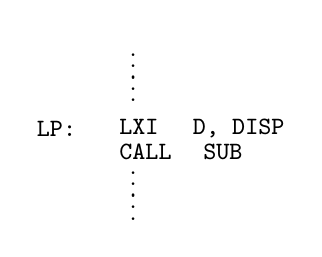
\begin{tikzpicture}[scale=0.6]
    % Labels and Assembly Code
    \node at (0, 1.5) {$\vdots$};
    \node at (0, 1) {$\vdots$};
    \node[left] at (-1, 0) {\texttt{LP:}};
    \node[right] at (-0.5, 0) {\texttt{LXI \hspace{3pt} D, DISP}};
    \node[right] at (-0.5, -0.5) {\texttt{CALL \hspace{2pt} SUB}};
    \node at (0, -1) {$\vdots$};
    \node at (0, -1.5) {$\vdots$};
\end{tikzpicture}
\end{center}

It is desired that control be returned to LP + DISP + 3 when the RET instruction is executed in the subroutine. The set of instructions that precede the RET instruction in the subroutine are
\begin{multicols}{4}
\begin{enumerate}
\item POP \hfill{D} \\ DAD \hfill{H}\\ PUSH \hfill{D} \\\\\\
\item  POP \hfill{H}\\ DAD \hfill{D}\\ INX \hfill{H}\\ INX \hfill{H}\\ INX \hfill{H}\\ PUSH \hfill{H}
\item  POP \hfill{H}\\ DAD \hfill{D}\\ PUSH \hfill{H}\\\\\\
\item XTHL\\ INX \hfill{D}\\ INX \hfill{D}\\ INX \hfill{D}\\ XTHL
\end{enumerate}
\end{multicols}

\item The transistor used in the circuit shown below has a $\beta$ of $30$ and $I_{CBO}$ is negligible.
\begin{center}
    
\begin{circuitikz}
\tikzstyle{every node}=[font=\normalsize]
\draw (4.25,6.25) to[Tnpn, transistors/scale=1.19] (4.25,8.75);
\draw (4.25,8.75) to[R] (4.25,10);
\draw (4.25,10) to[short] (0.25,10);
\draw (0.25,10) to[R] (0.25,7.5);
\draw (4.25,5.5) to[short] (0.25,5.5);
\draw (4.25,5.5) to[short, -o] (4.25,5) ;
\draw (1.75,7.5) to[D] (3.25,7.5);
\draw (1.75,7.5) to[R] (0.25,7.5);
\draw (0.25,5.5) to[empty Schottky diode] (0.25,7.5);
\draw (4.25,6.25) to[short] (4.25,5.5);
\node [font=\normalsize] at (-0.75,6.5) {$V_Z=5V$};
\node [font=\normalsize] at (-0.5,8.75) {$15k$};
\node [font=\normalsize] at (1,8) {$1 k$};
\node [font=\normalsize] at (2.5,8) {$D$};
\node [font=\normalsize] at (3.5,9.5) {$2.2k$};
\node [font=\normalsize] at (5,5) {$12V$};
\node [font=\normalsize] at (5.25,8) {$V_{BE}=0.7V$};
\node [font=\normalsize] at (5.25,7.5) {$V_{CE\brak{sat}}=0.2V$};
\draw (4.25,10) to[short] (5,10);
\draw (5,10) to (5,9.75) node[ground]{};
\end{circuitikz}
\end{center}

If the forward voltage drop of the diode is $0.7 V$, then the current through the collector will be:
\begin{multicols}{4} 
\begin{enumerate}
\item $168 mA$
\item  $108 mA$
\item  $20.54 mA$
\item $5.36 mA$
\end{enumerate}
\end{multicols}

\item 
A voltage commutated chopper circuit, operated at $500 Hz$, is shown below.
\begin{center}
\begin{circuitikz}
\tikzstyle{every node}=[font=\small]
\draw (9,9.5) to[european resistor] (9,7.25);
\draw (8,7.25) to[D] (8,9.5);
\draw (4.5,9.5) to[D] (5.5,9.5);
\draw (4.5,8.75) to[D] (5.5,8.75);
\draw (6.5,8) to[D] (5.5,8);
\draw (4,8) to[L ] (5.5,8);
\draw (6.5,9.5) to[short] (8.25,9.5);
\draw (6.5,9.5) to[short] (6.5,8);
\draw (4,9.5) to[C] (4,8.75);
\draw (4,8.75) to[short] (4,8);
\draw [->, >=Stealth] (5.5,9.5) -- (6,9.5);
\draw [->, >=Stealth] (5.5,8.75) -- (6,8.75);
\draw [short] (6,9.5) -- (6.5,9.5);
\draw [short] (6,8.75) -- (6.5,8.75);
\draw [<->, >=Stealth] (2.75,9.25) -- (2.75,7.5);
\draw (4.5,9.5) to[short, -o] (2.75,9.5) ;
\draw (9,7.25) to[short, -o] (2.75,7.25) ;
\node [font=\normalsize] at (2.25,8.5) {200V};
\node [font=\small] at (3.5,8.75) {0.1uF};
\node [font=\small] at (4.75,7.5) {1mH};
\node [font=\small] at (6,9) {$i_A$};
\node [font=\small] at (6,10) {$i_M$};
\node [font=\small] at (5.5,9) {M};
\node [font=\footnotesize] at (5.25,10) {A};
\node [font=\normalsize] at (9.75,8.5) {LOAD};
\node [font=\small] at (8.5,10) {$i_L=10A$};
\draw [->, >=Stealth] (8.25,9.5) -- (8.75,9.5);
\draw [short] (8.75,9.5) -- (9,9.5);
\draw [short] (4,8.75) -- (4.5,8.75);
\end{circuitikz}
\end{center}

If the maximum value of load current is $10 A$, then the maximum current through the main (M) and auxiliary (A) thyristors will be:
\begin{multicols}{2}
\begin{enumerate}
\item $i_{M \text{max }} = 12\,A \text{ and } i_{A \text{max }} = 10\,A$
\item  $i_{M \text{max }} = 12\,A \text{ and } i_{A \text{max }} = 2\,A$
\item  $i_{M \text{max }} = 10\,A \text{ and } i_{A \text{max }} = 12\,A$
\item $i_{M \text{max }} = 10\,A \text{ and } i_{A \text{max }} = 8\,A$
\end{enumerate}
\end{multicols}

\item The matrix $\sbrak{A}=\myvec{2 & 1 \\ 4 & -1}$ is decomposed into a product of a lower triangular matrix $\sbrak{L}$ and an upper triangular matrix $\sbrak{U}$. The properly decomposed $\sbrak{L}$ and $\sbrak{U}$ matrices respectively are
\begin{multicols}{2}
\begin{enumerate}
\item $\myvec{1 & 0 \\ 4 & -1} \text{ and } \myvec{1 & 1 \\ 0 & -2 }$
\item $\myvec{2 & 0 \\ 4 & -1} \text{ and } \myvec{1 & 1 \\ 0 & 1 }$
\item $\myvec{1 & 0 \\ 4 & 1} \text{ and } \myvec{2& 1 \\ 0 & -1 }$
\item $\myvec{2 & 0 \\ 4 & -3} \text{ and } \myvec{1 & 0.5 \\ 0 & 1 }$
\end{enumerate}
\end{multicols}


\item The two vectors $\myvec{1\\ 1\\ 1}$ and $\myvec{1\\ a\\ a^2}$, where $a = \brak{ \frac{1}{2} + j\frac{\sqrt{3}}{2} }$, are
\begin{multicols}{4}
\begin{enumerate}
\item orthonormal
\item  orthonormal
\item  parallel
\item  collinear
\end{enumerate}
\end{multicols}

\item A three-phase $440V, 6 \text{ pole }, 50Hz,$ squirrel cage induction motor is running at a slip of $5\%$. The speed of stator magnetic field with respect to rotor magnetic field and speed of rotor with respect to stator magnetic field are
\begin{multicols}{2}
\begin{enumerate}
\item $0, -5 rpm$
\item  $0, 955 rpm$
\item  $1000 rpm, -5 rpm$
\item $1000 rpm, 955 rpm$
\end{enumerate}
\end{multicols}



